\topic{7.3 continued}{Case A: prescribed source and boundary data}
Consider one Poisson solve on the unit square. Its equation and data are
\[
\nabla^2\psi=-\omega,\qquad
\omega=-2\ \hbox{at the interior nodes},\qquad
\psi=0\ \hbox{at every boundary node}.
\]
Vorticity is prescribed at the four interior nodes. Their streamfunction
values are the unknowns in this Poisson problem.

\textbf{Zero boundary values do not mean a zero interior solution.}
The equation has a nonzero right side: $-\omega=2$. Setting $\psi=0$
everywhere would give $\nabla^2\psi=0$, which would not satisfy that equation.
If both the boundary data and the prescribed vorticity were zero, the solution
would instead be zero everywhere.

\textbf{Locate the four unknowns.} There are four grid coordinates in each
direction, $0,1/3,2/3,1$. Hence $h=1/3$ and $h^2=1/9$.
The outer twelve grid nodes are prescribed; only the four interior nodes remain:
\begin{center}
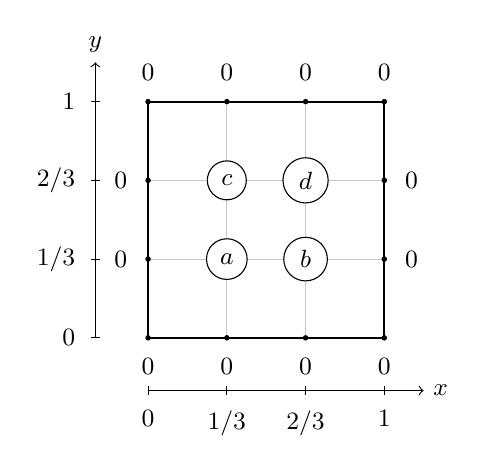
\begin{tikzpicture}[x=10mm,y=10mm,every node/.style={font=\small}]
\foreach \j in {0,1,2,3} {
  \draw[gray!45,thin] (0,\j)--(3,\j);
  \draw[gray!45,thin] (\j,0)--(\j,3);
}
\draw[thick] (0,0) rectangle (3,3);
\foreach \i in {0,1,2,3} {
  \fill (\i,0) circle (0.035);
  \fill (\i,3) circle (0.035);
  \node[below=4pt] at (\i,0) {$0$};
}
\foreach \j in {1,2} {
  \fill (0,\j) circle (0.035);
  \fill (3,\j) circle (0.035);
  \node[left=4pt] at (0,\j) {$0$};
  \node[right=4pt] at (3,\j) {$0$};
}
\foreach \i in {0,2,3} {\node[above=4pt] at (\i,3) {$0$};}
\node[above=4pt] at (1,3) {$0$};

\node[draw,circle,fill=white,inner sep=3pt] at (1,1) {$a$};
\node[draw,circle,fill=white,inner sep=3pt] at (2,1) {$b$};
\node[draw,circle,fill=white,inner sep=3pt] at (1,2) {$c$};
\node[draw,circle,fill=white,inner sep=3pt] at (2,2) {$d$};
\draw[->] (0,-.67)--(3.5,-.67) node[right] {$x$};
\draw[->] (-.67,0)--(-.67,3.5) node[above] {$y$};
\foreach \i/\value in {0/0,1/{1/3},2/{2/3},3/1} {
 \draw (\i,-.61)--(\i,-.73);
 \node[below=2pt] at (\i,-.73) {$\value$};
 \draw (-.61,\i)--(-.73,\i);
 \node[left=2pt] at (-.73,\i) {$\value$};
}
\end{tikzpicture}
\end{center}
\[
\begin{aligned}
a&=\psi(1/3,1/3),& b&=\psi(2/3,1/3),\\
c&=\psi(1/3,2/3),& d&=\psi(2/3,2/3).
\end{aligned}
\]

\textbf{Apply the same stencil at each unknown.} From the preceding derivation,
\[
4\psi_C-\psi_E-\psi_W-\psi_N-\psi_S=h^2\omega_C=-2/9.
\]
The sign is worth checking: the PDE is $\nabla^2\psi=2$, whereas the
positive-center stencil above represents $-h^2\nabla^2\psi$.
Substitution of each node's actual neighbors gives
\begin{align*}
4a-\underbrace{b}_{E}-\underbrace{0}_{W}-\underbrace{c}_{N}-\underbrace{0}_{S}&=-2/9,\\
4b-\underbrace{0}_{E}-\underbrace{a}_{W}-\underbrace{d}_{N}-\underbrace{0}_{S}&=-2/9,\\
4c-\underbrace{d}_{E}-\underbrace{0}_{W}-\underbrace{0}_{N}-\underbrace{a}_{S}&=-2/9,\\
4d-\underbrace{0}_{E}-\underbrace{c}_{W}-\underbrace{0}_{N}-\underbrace{b}_{S}&=-2/9.
\end{align*}
Every boundary zero is known data. Every letter on a neighboring interior node
must be retained as an unknown.
\newpage
\topic{7.3 continued}{Case A: discrete system and solution}
Choose the unknown order $(a,b,c,d)$ once, and use it in every row:
\[
\underbrace{\begin{bmatrix}
4&-1&-1&0\\-1&4&0&-1\\-1&0&4&-1\\0&-1&-1&4
\end{bmatrix}}_{M}
\underbrace{\begin{bmatrix}a\\b\\c\\d\end{bmatrix}}_{\boldsymbol q_A}
=\underbrace{\begin{bmatrix}-2/9\\-2/9\\-2/9\\-2/9\end{bmatrix}}_{\boldsymbol r_A}.
\]
The matrix $M$ records which interior nodes are neighbors. The vector
$\boldsymbol r_A$ contains the known source and boundary contributions.


\begin{center}\begin{tabular}{cll}\toprule
Row & Interior neighbors & Equation\\\midrule
$a$ & $b,c$ & $4a-b-c=-2/9$\\
$b$ & $a,d$ & $-a+4b-d=-2/9$\\
$c$ & $a,d$ & $-a+4c-d=-2/9$\\
$d$ & $b,c$ & $-b-c+4d=-2/9$\\\bottomrule
\end{tabular}\end{center}
For instance, the zero in row 1, column 4 means that $d$ is diagonal to $a$;
it is not a neighbor in the five-point stencil. The boundary zeros are absent
from $M$ because their values are already known.

\textbf{Solve this symmetric case.} The square, source and boundary data treat
the four interior positions identically. The unique discrete solution must
therefore have $a=b=c=d=s$. Each row reduces to
\[
4s-s-s=-2/9\quad\Longrightarrow\quad 2s=-2/9
\quad\Longrightarrow\quad \boxed{s=-1/9\simeq-0.111111.}
\]
Check by substitution, for example at $a$:
\[
4(-1/9)-(-1/9)-(-1/9)=-2/9.
\]
The other three rows give the same result. Equivalently, at each interior node,
\[
\frac{\psi_E+\psi_W+\psi_N+\psi_S-4\psi_C}{h^2}
=\frac{2/9}{1/9}=2=-\omega_C.
\]
This is the exact answer to this \emph{discrete} four-unknown problem. It is
not an assertion that the continuum solution is constant throughout the square:
the boundary nodes remain zero, and a finer grid contains more interior values.

\checkpoint{Keep $h=1/3$ and the zero boundaries, but set the prescribed
vorticity to $-1$. What changes in $M$, in the right side, and in the answer?
The matrix is unchanged, the right side halves, and each interior value is $-1/18$.}
\newpage
\topic{7.3 continued}{Case A: Jacobi iteration}
Direct solution of $M\boldsymbol q_A=\boldsymbol r_A$ is convenient for four
unknowns. Jacobi iteration illustrates the procedure used on a larger grid.
Isolate the central value in each row:
\begin{align*}
a^{k+1}&=\tfrac14(b^k+c^k-2/9),&
b^{k+1}&=\tfrac14(a^k+d^k-2/9),\\
c^{k+1}&=\tfrac14(a^k+d^k-2/9),&
d^{k+1}&=\tfrac14(b^k+c^k-2/9).
\end{align*}
The superscript $k$ counts solver sweeps. All four new values must use only
values from sweep $k$. Initialize the interior guesses to zero; these guesses
are not additional boundary conditions.

\textbf{First sweep.} Both interior neighbors are still zero:
\[
a^1=b^1=c^1=d^1=\tfrac14(0+0-2/9)=-1/18.
\]
\textbf{Second sweep.} Both neighbors now have the previous value $-1/18$:
\[
a^2=\tfrac14(-1/18-1/18-2/9)=-1/12.
\]
By symmetry, the other three entries again equal $a^2$.
\begin{center}\begin{tabular}{rrr}\toprule
Sweep $k$ & Each interior value & Absolute error relative to $-1/9$\\\midrule
0 & $0$ & $1/9$\\
1 & $-1/18$ & $1/18$\\
2 & $-1/12$ & $1/36$\\
3 & $-7/72$ & $1/72$\\
$\infty$ & $-1/9$ & $0$\\\bottomrule
\end{tabular}\end{center}
The error halves per sweep in this symmetric example. That factor is a property
of this tiny system and starting guess; it is not a universal rate for Jacobi.

\textbf{Connection to the code.} The assignment \texttt{old = psi.copy()}
preserves the previous sweep. Four neighbor slices of \texttt{old} supply the
new interior values. Reusing a newly computed neighbor within the same sweep
would be a different algorithm, such as Gauss--Seidel.

\textbf{What stays fixed?} During this Poisson solve, $h$, $\omega$, boundary
data and physical time stay fixed. Only the interior guesses change. A cavity
time step later changes vorticity and requires another Poisson solve.

Case A is now complete. Its final answer is $(-1/9,-1/9,-1/9,-1/9)$.
The next page introduces different boundary data in a separate problem.
\newpage
\topic{7.3 continued}{Case B: a nonzero boundary value}
\textbf{Change one prescribed value, and nothing else.}
Retain the square, the grid spacing $h=1/3$, the four unknown positions and
$\omega=-2$. Introduce a known boundary value
\[
\boxed{g=\psi(1/3,1)=0.1.}
\]
This is the north neighbor of $c$. All other boundary nodes remain zero:
\begin{center}
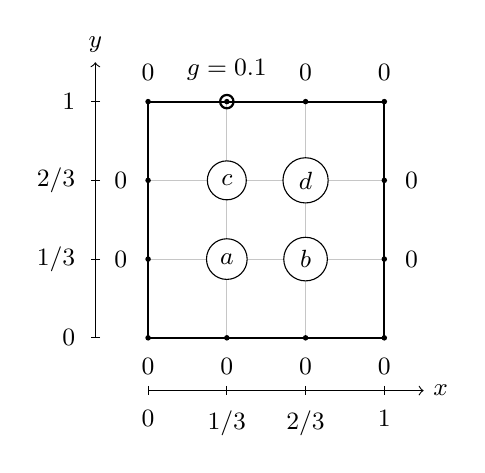
\begin{tikzpicture}[x=10mm,y=10mm,every node/.style={font=\small}]
\foreach \j in {0,1,2,3} {
  \draw[gray!45,thin] (0,\j)--(3,\j);
  \draw[gray!45,thin] (\j,0)--(\j,3);
}
\draw[thick] (0,0) rectangle (3,3);
\foreach \i in {0,1,2,3} {
  \fill (\i,0) circle (0.035);
  \fill (\i,3) circle (0.035);
  \node[below=4pt] at (\i,0) {$0$};
}
\foreach \j in {1,2} {
  \fill (0,\j) circle (0.035);
  \fill (3,\j) circle (0.035);
  \node[left=4pt] at (0,\j) {$0$};
  \node[right=4pt] at (3,\j) {$0$};
}
\foreach \i in {0,2,3} {\node[above=4pt] at (\i,3) {$0$};}
\node[above=4pt] at (1,3) {$g=0.1$};
\draw[thick] (1,3) circle (0.085);
\node[draw,circle,fill=white,inner sep=3pt] at (1,1) {$a$};
\node[draw,circle,fill=white,inner sep=3pt] at (2,1) {$b$};
\node[draw,circle,fill=white,inner sep=3pt] at (1,2) {$c$};
\node[draw,circle,fill=white,inner sep=3pt] at (2,2) {$d$};
\draw[->] (0,-.67)--(3.5,-.67) node[right] {$x$};
\draw[->] (-.67,0)--(-.67,3.5) node[above] {$y$};
\foreach \i/\value in {0/0,1/{1/3},2/{2/3},3/1} {
 \draw (\i,-.61)--(\i,-.73);
 \node[below=2pt] at (\i,-.73) {$\value$};
 \draw (-.61,\i)--(-.73,\i);
 \node[left=2pt] at (-.73,\i) {$\value$};
}
\end{tikzpicture}
\end{center}
The circled boundary node prescribes $\psi=g=0.1$ directly above $c$.

\textbf{Revisit the row that touches this boundary node.} At $c$, the stencil is
\begin{align*}
4c-\underbrace{d}_{E}-\underbrace{0}_{W}
-\underbrace{g}_{N}-\underbrace{a}_{S}&=-2/9,\\
-a+4c-d&=-2/9+g.
\end{align*}
The known term $-g$ moves to the right with a plus sign. None of the other
three rows directly touches this changed boundary node, so their right sides
remain $-2/9$. Hence
\[
M\boldsymbol q_B=\boldsymbol r_B,
\qquad
\boldsymbol r_B=\begin{bmatrix}-2/9\\-2/9\\-2/9+0.1\\-2/9\end{bmatrix}
=\begin{bmatrix}-2/9\\-2/9\\-11/90\\-2/9\end{bmatrix}.
\]
The matrix is still the same $M$: the interior connectivity has not changed.
Only entry 3 of the right side changes \emph{directly}. The coupled solve can
nevertheless change all four interior values.

This boundary perturbation is an algebraic Poisson exercise. A spatially varying
wall streamfunction does not describe the original impermeable cavity wall,
whose streamfunction is constant. Use the original cavity boundary conditions
again when returning to the flow solver.
\newpage
\topic{7.3 continued}{Case B: solution and boundary response}
Let $\delta\boldsymbol q=\boldsymbol q_B-\boldsymbol q_A$ be the change in the
four interior values. Subtract the two systems:
\[
M\delta\boldsymbol q=\boldsymbol r_B-\boldsymbol r_A
=\begin{bmatrix}0\\0\\g\\0\end{bmatrix}.
\]
The first and fourth rows have the same neighbor terms. Subtracting them gives
$4(\delta a-\delta d)=0$, so $\delta a=\delta d$. Write this shared value as
$t$. The four rows reduce to three distinct equations:
\[
4t-\delta b-\delta c=0,\qquad
4\delta b-2t=0,\qquad
4\delta c-2t=g.
\]
The second equation gives $\delta b=t/2$; the third gives
$\delta c=g/4+t/2$. Substitute them into the first:
\[
4t-t/2-(g/4+t/2)=0
\quad\Longrightarrow\quad 3t=g/4
\quad\Longrightarrow\quad t=g/12.
\]
Therefore
\[
\delta a=\delta d=g/12,\qquad
\delta b=g/24,\qquad \delta c=7g/24.
\]
For $g=0.1$, add these changes to the Case A answer:
\begin{center}\begin{tabular}{cccc}\toprule
Unknown & Case A & Change & Case B\\\midrule
$a$ & $-1/9$ & $+1/120$ & $-37/360\simeq-0.102778$\\
$b$ & $-1/9$ & $+1/240$ & $-77/720\simeq-0.106944$\\
$c$ & $-1/9$ & $+7/240$ & $-59/720\simeq-0.081944$\\
$d$ & $-1/9$ & $+1/120$ & $-37/360\simeq-0.102778$\\\bottomrule
\end{tabular}\end{center}
The largest change is at $c$, which directly touches the perturbed boundary.
The other nodes respond through their interior neighbors. For a check of the
modified row, use denominator 720:
\[
4c-a-d=\frac{-236+74+74}{720}
=-\frac{88}{720}=-\frac{11}{90}=-2/9+0.1.
\]
Jacobi can solve Case B as well: use the same four updates as before, but add
$g$ only inside the parentheses of the $c$ update. Starting from zero, the first
sweep gives $a^1=b^1=d^1=-1/18$ and $c^1=-11/360$.

\checkpoint{If $g$ changes from $0.1$ to $0.2$, which matrix entries change?
None. The boundary contribution doubles, so every entry of
$\boldsymbol q_B-\boldsymbol q_A$ doubles. The Case A solution itself does not double.}
